\begin{frame}[fragile]
\frametitle{Аллокация памяти}
\begin{itemize}
    \item<1->Рассмотрим простейшую постановку задачи:
    \begin{itemize}
        \item<2->есть непрерывный участок логической памяти;
        \item<3->функция аллокации: \lstinline|void *alloc(int size)|;
        \item<4->функция освобождения: \lstinline|void free(void *free)|.
    \end{itemize}
\end{itemize}
\end{frame}

\begin{frame}
\frametitle{Выравнивание}
\begin{itemize}
    \item<1->Некоторые процессоры требуют выравненных указателей
    \begin{itemize}
        \item<2->2 байта - выравнивание 2 байта;
        \item<3->4 байта - выравнивание 4 байта;
        \item<4->8 байт - выравнивание 8 байт...
    \end{itemize}
\end{itemize}
\end{frame}

\begin{frame}
\frametitle{Простой подход к аллокации}
\begin{itemize}
    \item<1->Создадим связный список свободных блоков
    \begin{itemize}
        \item<1->каждый узел списка описывает непрерывный свободный участок;
        \item<2->узлы списка хранятся в начале каждого свободного блока.
    \end{itemize}
\end{itemize}
\end{frame}

\begin{frame}
\frametitle{Связный список свободных блоков}
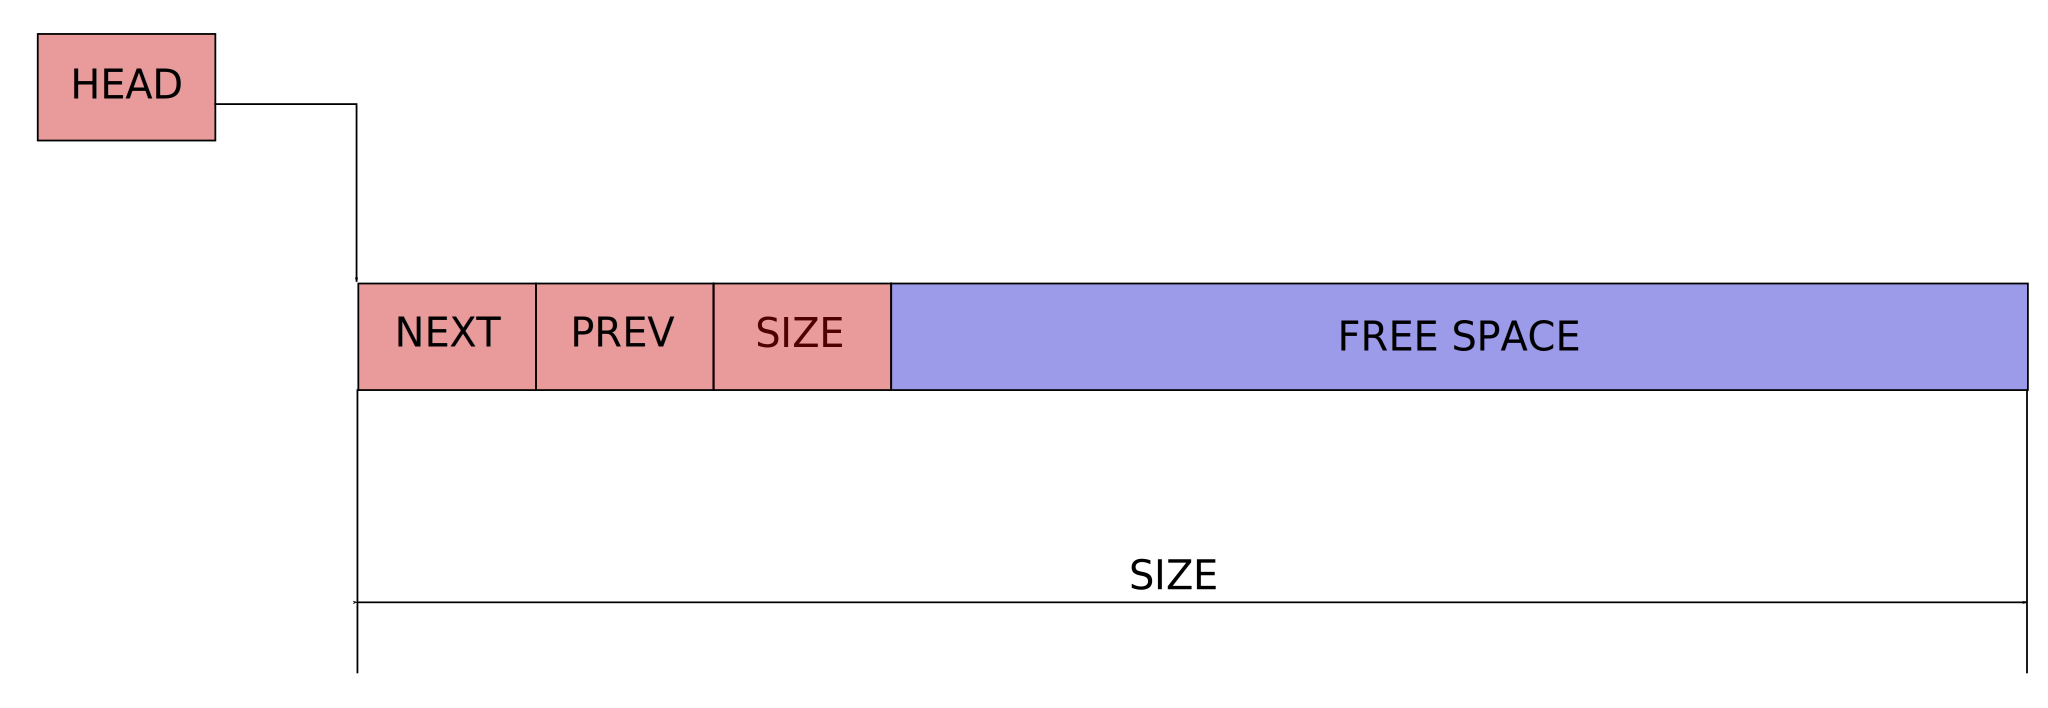
\includegraphics[height=.3\textheight]{lst0}
\end{frame}

\begin{frame}
\frametitle{Аллокация свободного блока}
\begin{itemize}
    \item<1->Пройдемся по списку и найдем блок достаточного размера
    \begin{itemize}
        \item<2->если блок слишком большой, то отрезаем от него часть;
        \item<3->если походящего блока не нашлось, то возвращаем ошибку.
    \end{itemize}
\end{itemize}
\end{frame}

\begin{frame}
\frametitle{Аллокация свободного блока}
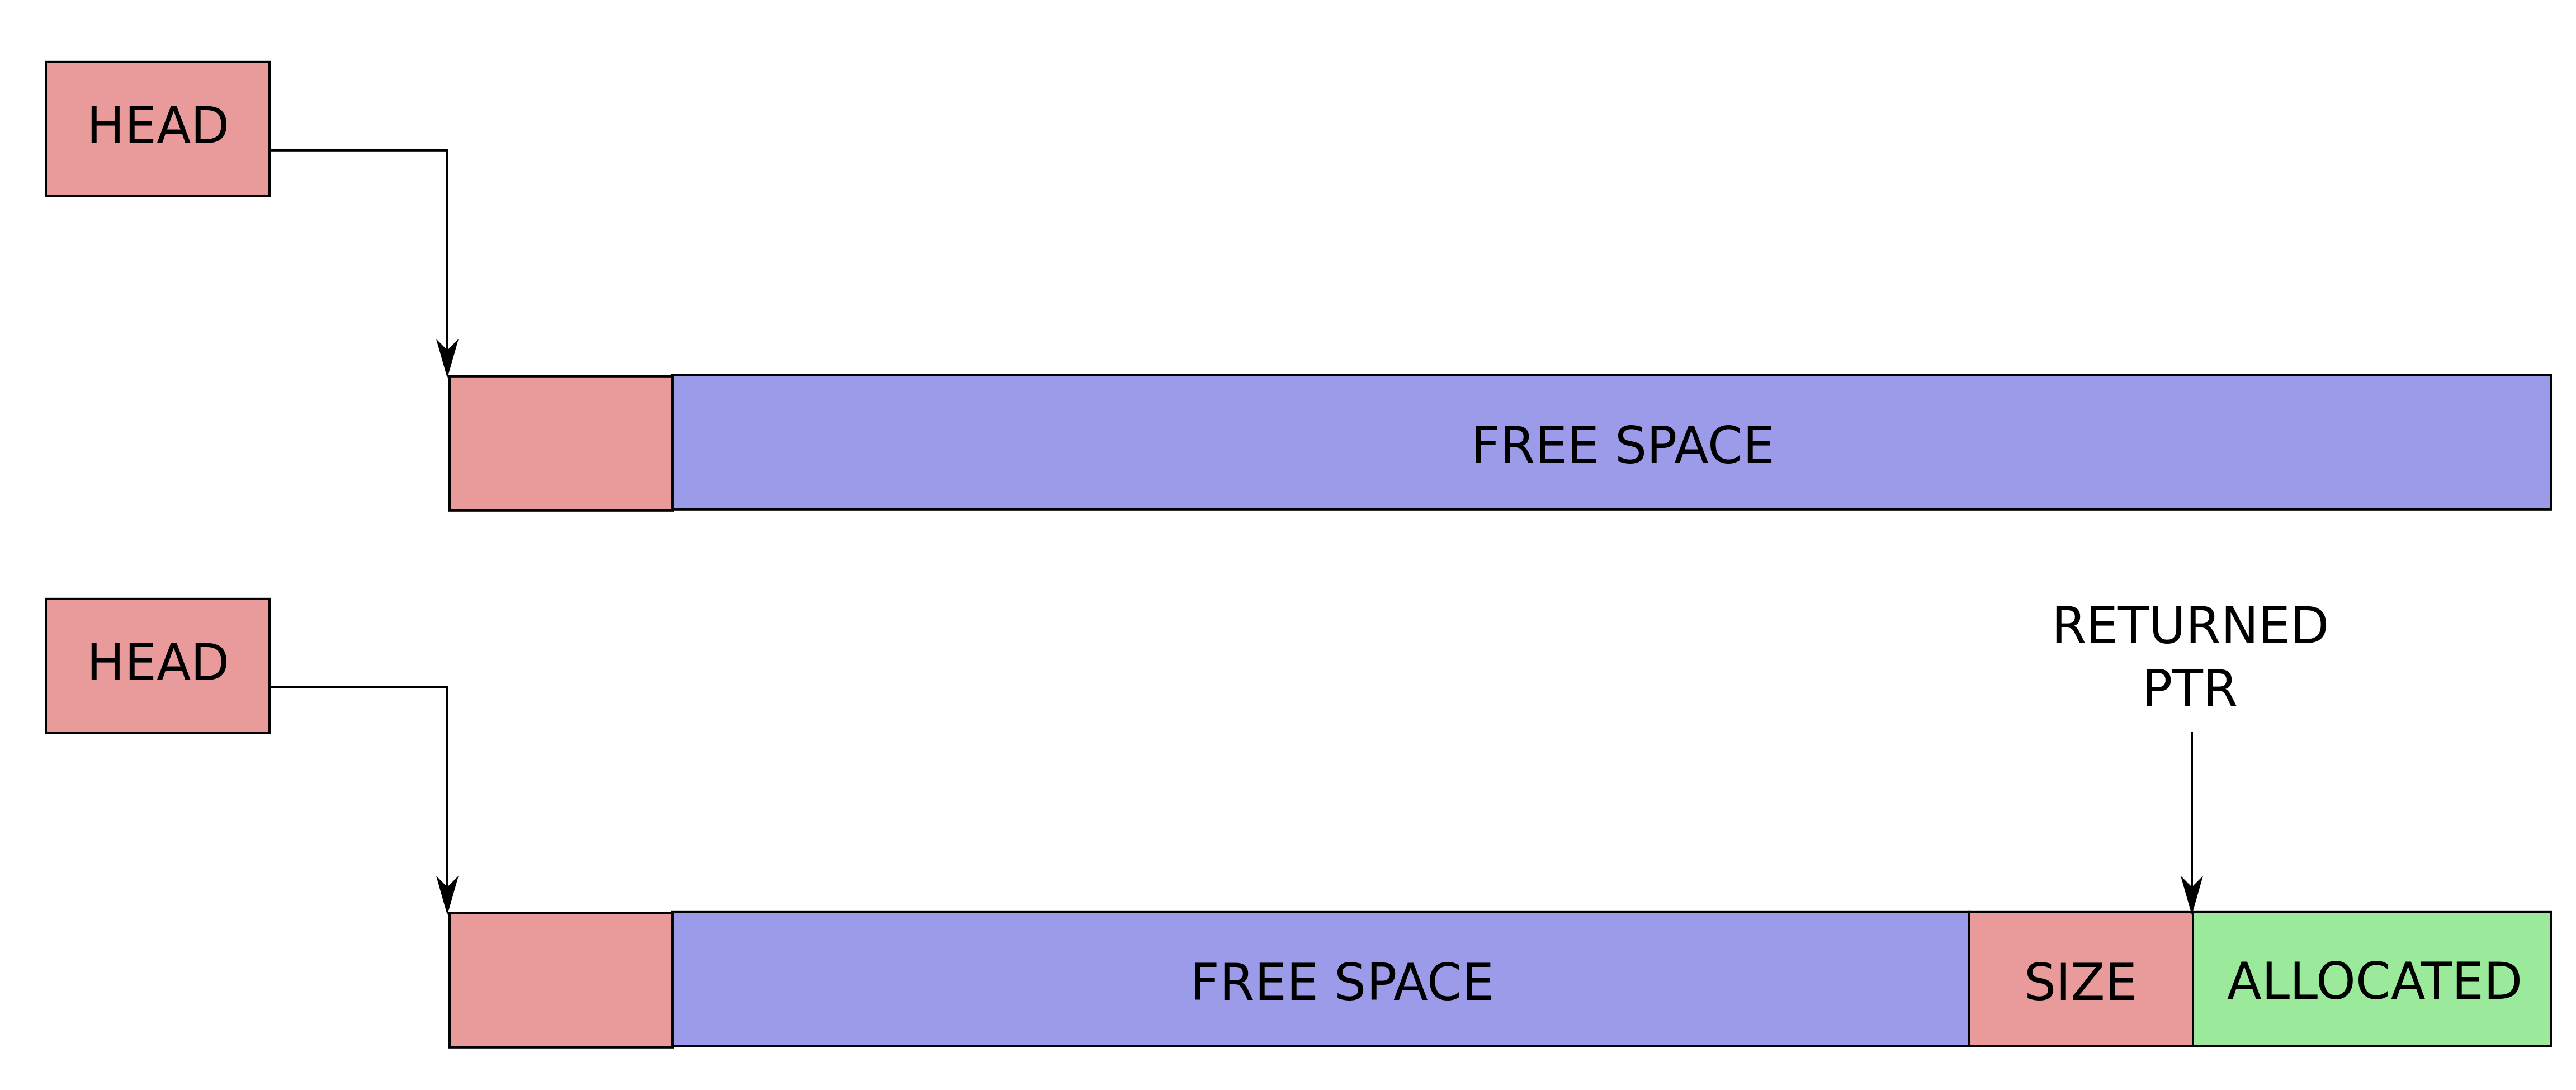
\includegraphics[height=.4\textheight]{lst1}
\end{frame}

\begin{frame}
\frametitle{Освобождение занятого блока}
\begin{itemize}
    \item<1->Чтобы освободить свободный блок его нужно вернуть в список
    \begin{itemize}
        \item<2->например, можно добавить в список новый элемент.
    \end{itemize}
\end{itemize}
\end{frame}

\begin{frame}
\frametitle{Освобождение занятого блока}
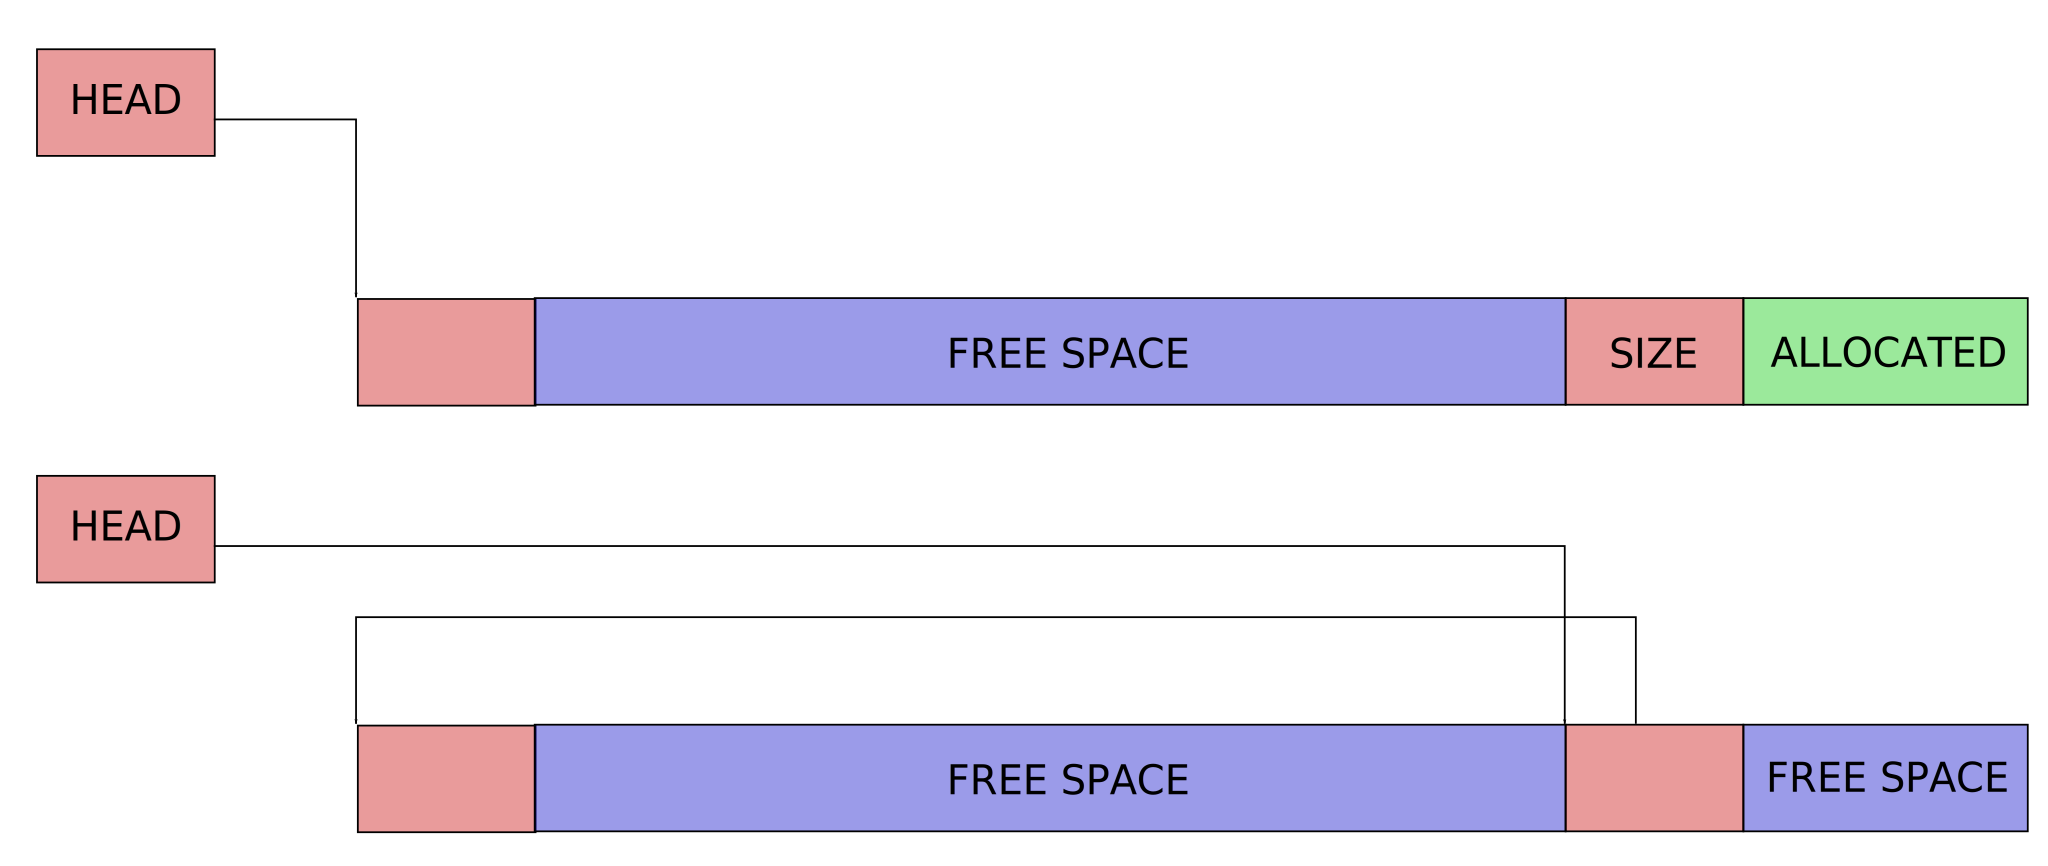
\includegraphics[height=.4\textheight]{lst2}
\end{frame}

\begin{frame}
\frametitle{Фрагментация свободной памяти}
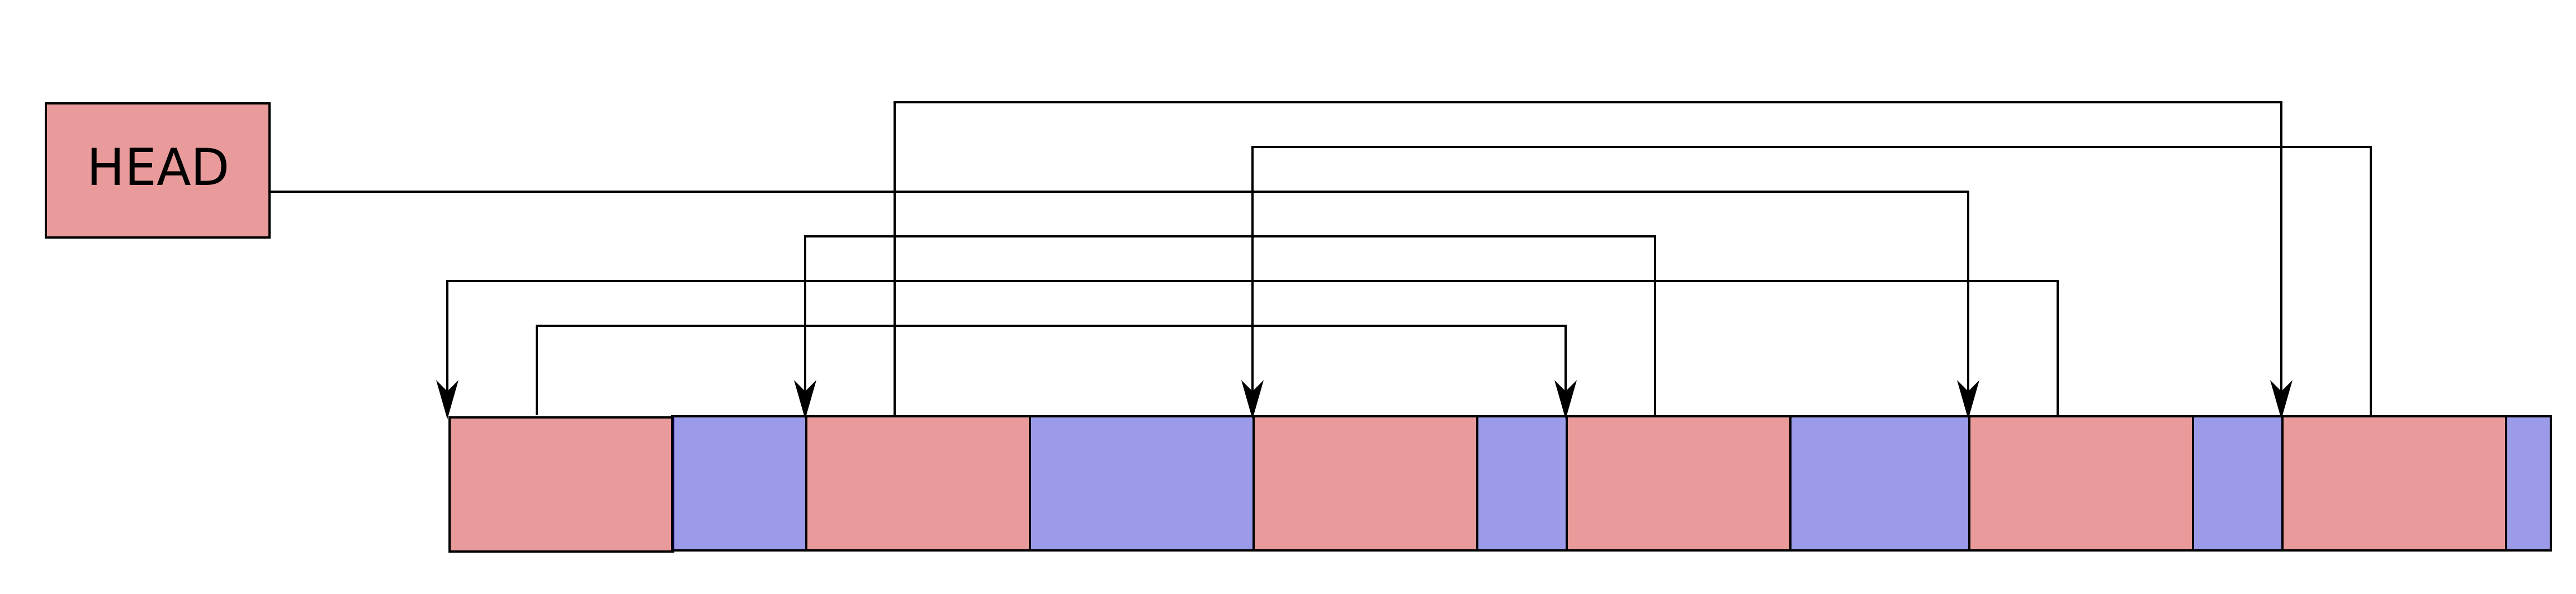
\includegraphics[height=.2\textheight]{lst3}
\end{frame}

\begin{frame}
\frametitle{Боремся с фрагментацией}
\begin{itemize}
    \item<1->Как избежать подобной фрагментации?
    \begin{itemize}
        \item<2->искать смежные блоки проходом по списку ($O\left(N\right)$);
        \item<3->поддерживать список упорядоченным ($O\left(N\right)$);
        \item<4->использовать упорядоченную структуру вместо списка
        ($O\left(log N\right)$);
        \item<5->использовать граничные маркеры (Border Tags,
        $O\left(1\right)$).
    \end{itemize}
\end{itemize}
\end{frame}

\begin{frame}
\frametitle{Граничные маркеры}
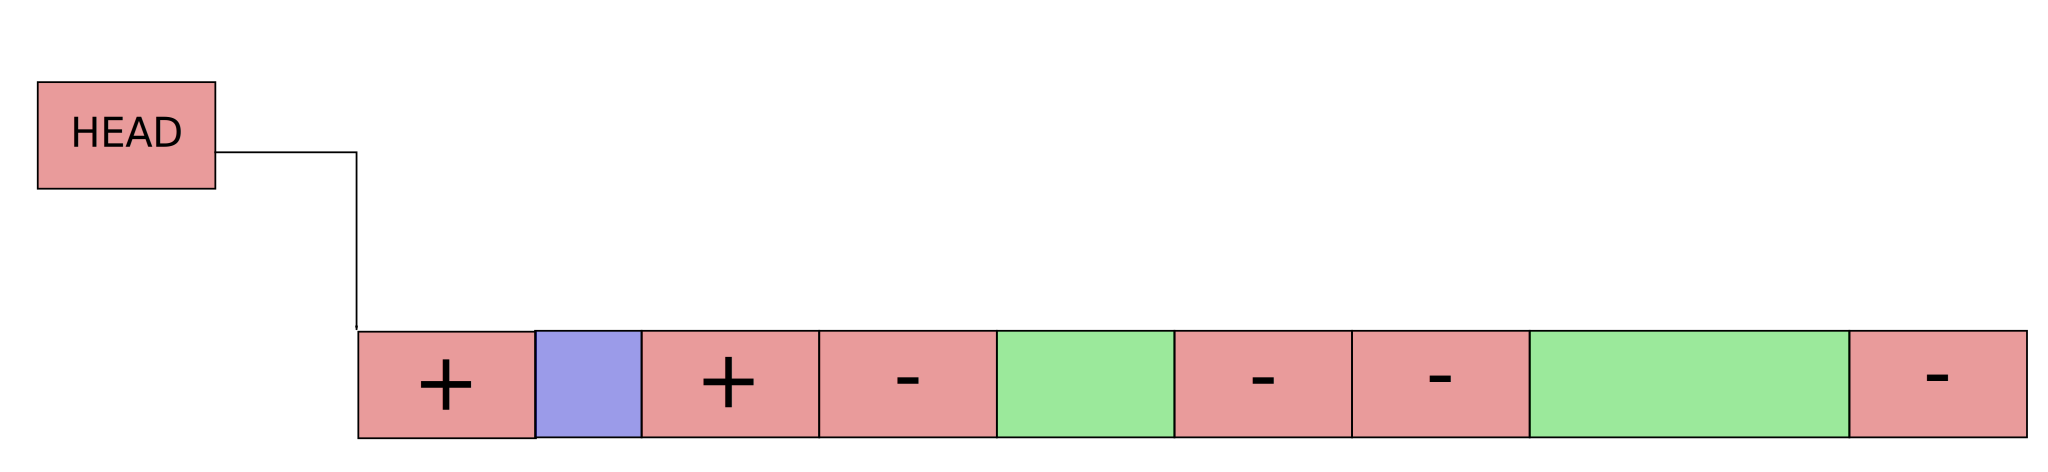
\includegraphics[height=.2\textheight]{lst4}
\end{frame}

\begin{frame}
\frametitle{Граничные маркеры}
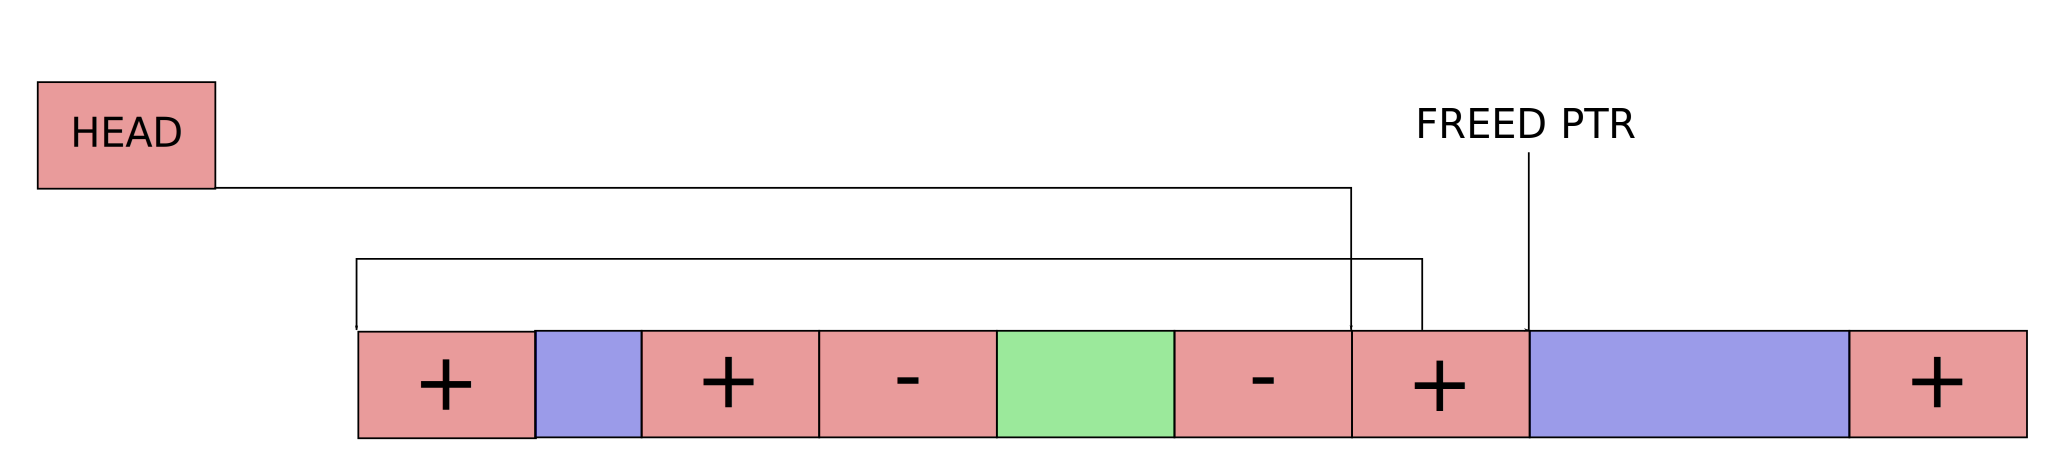
\includegraphics[height=.2\textheight]{lst5}
\end{frame}

\begin{frame}
\frametitle{Граничные маркеры}
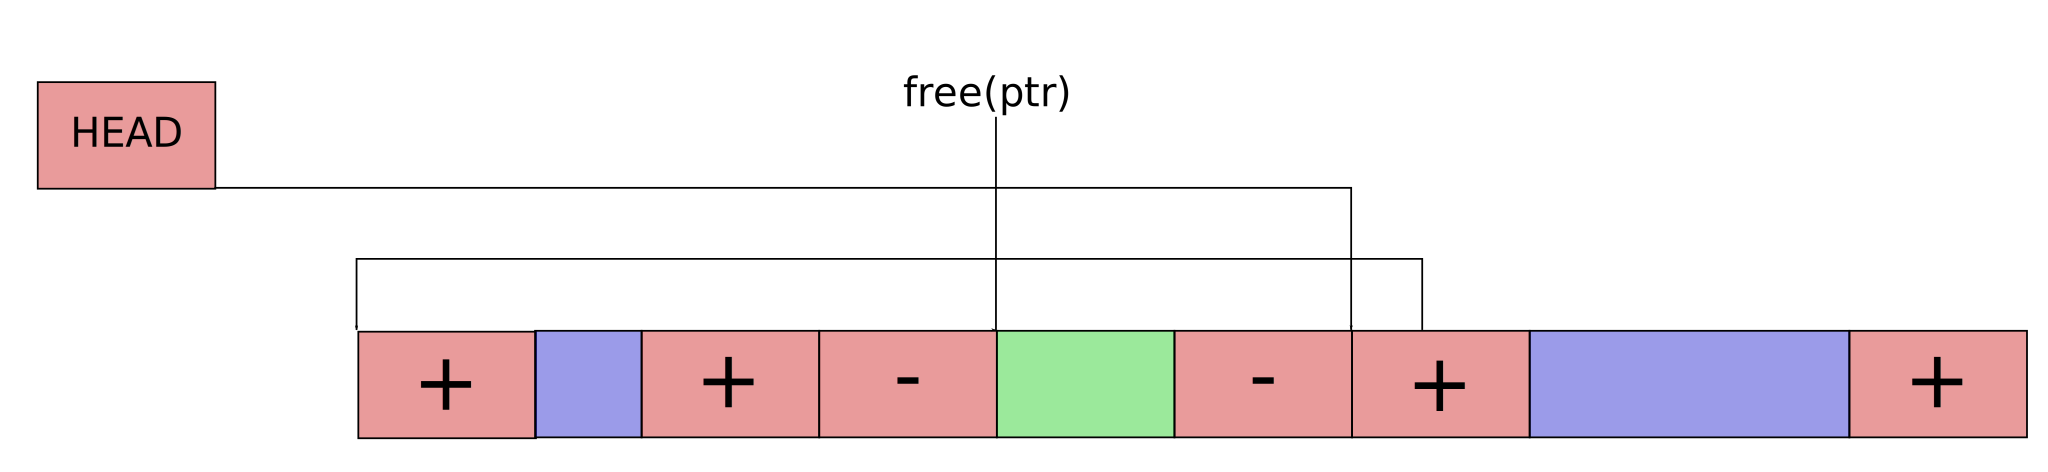
\includegraphics[height=.2\textheight]{lst6}
\end{frame}

\begin{frame}
\frametitle{Граничные маркеры}
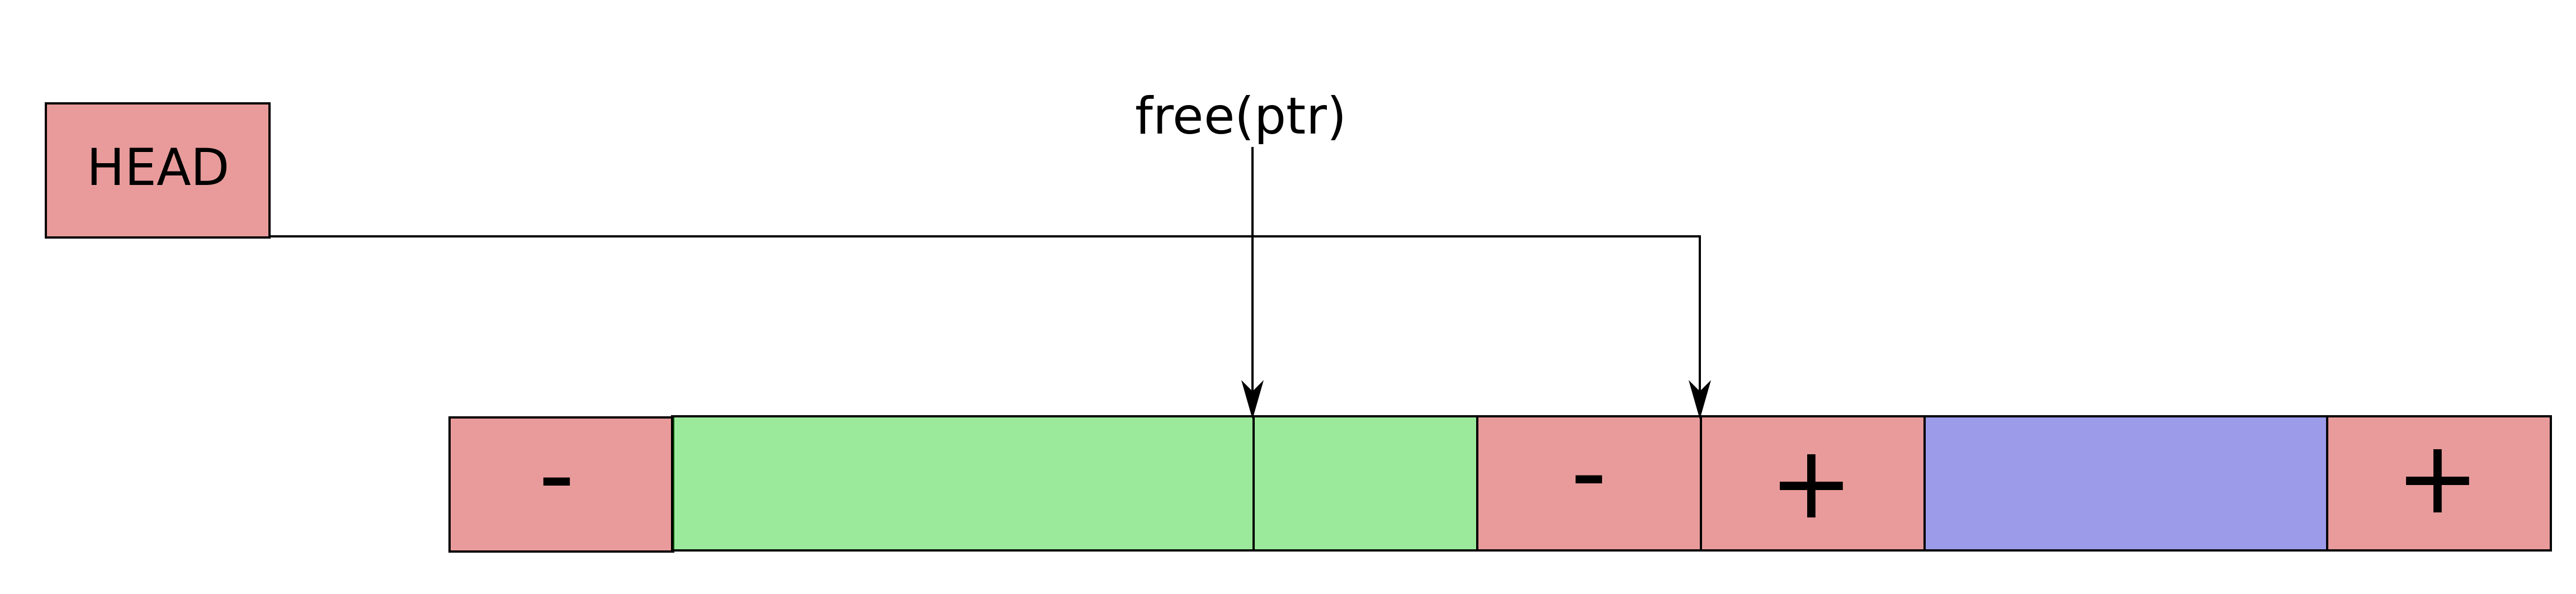
\includegraphics[height=.2\textheight]{lst7}
\end{frame}

\begin{frame}
\frametitle{Граничные маркеры}
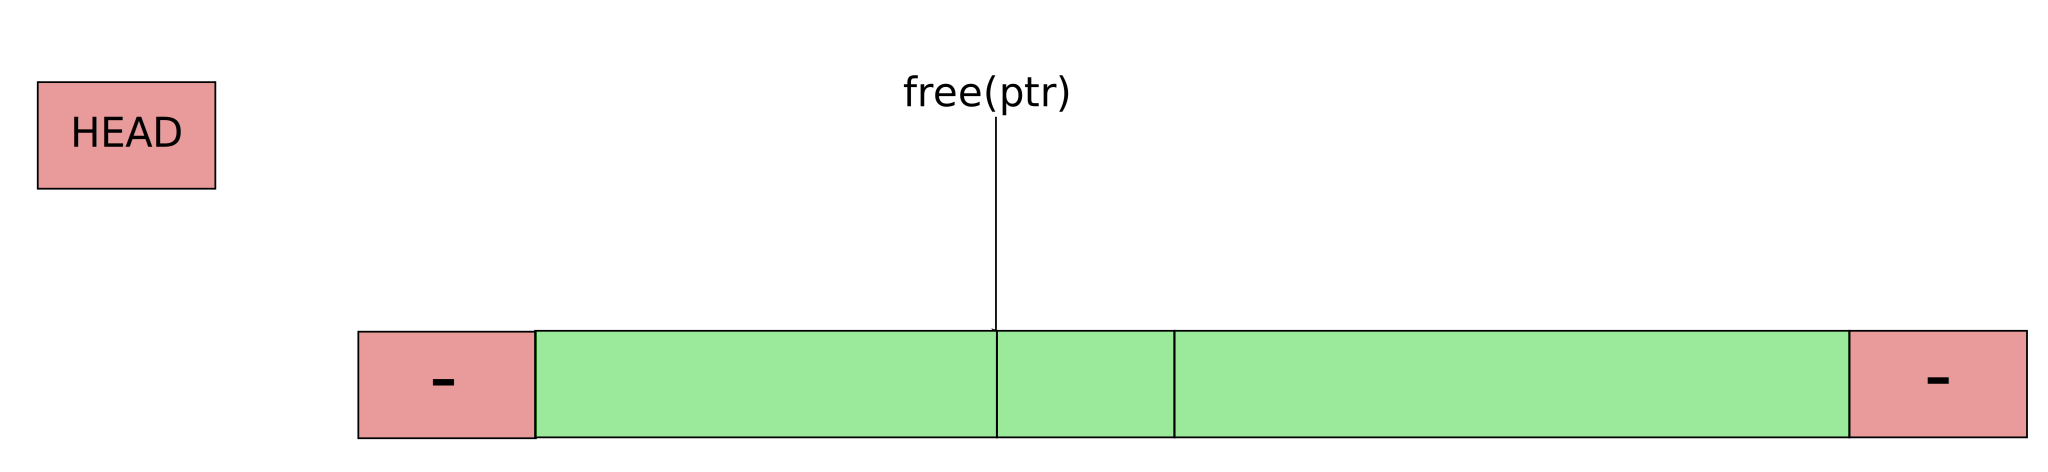
\includegraphics[height=.2\textheight]{lst8}
\end{frame}

\begin{frame}
\frametitle{Граничные маркеры}
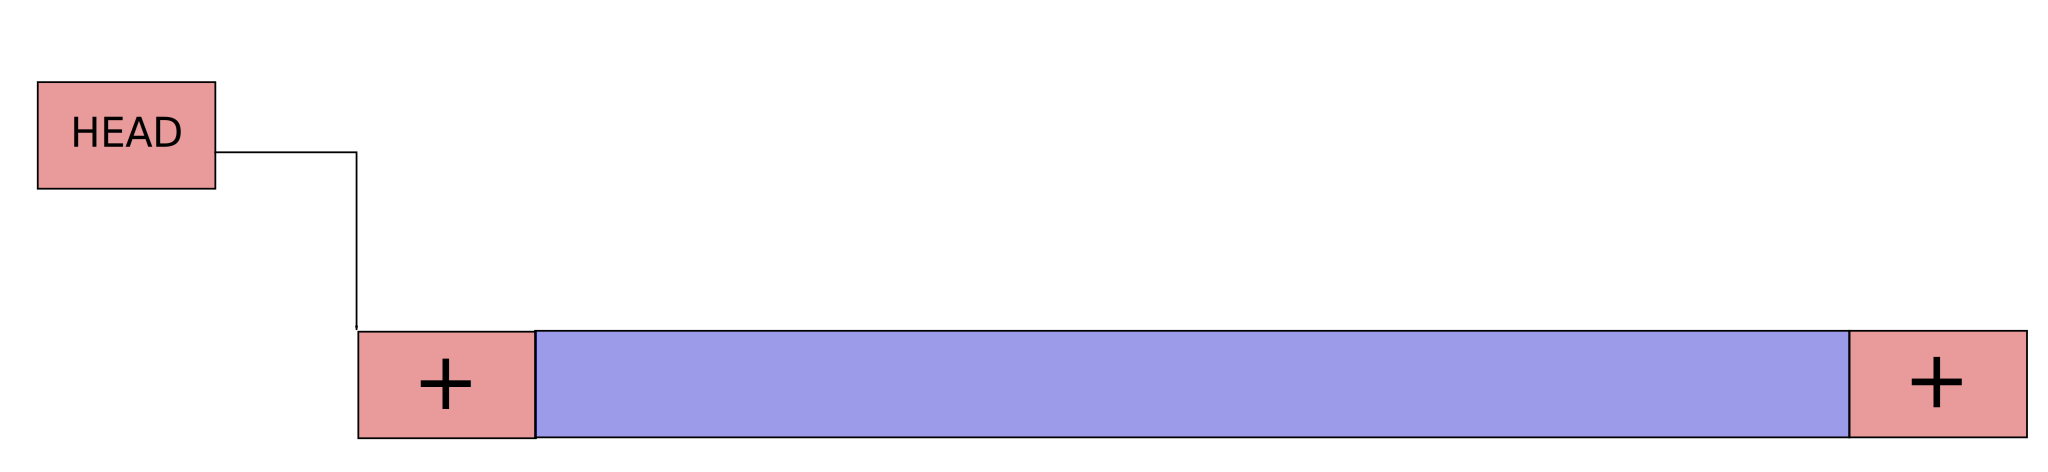
\includegraphics[height=.2\textheight]{lst9}
\end{frame}

